%!TEX root = thesis.tex
\chapter{Thermal Transport in Nanotubes }
\label{chap:nt}
\section{Introduction}\blfootnote{Portions of this chapter have originally been published in \cite{ownNT} ``Thermal Transport in Semiconductor Nanotubes" (2019), \textit{International Journal of Heat and Mass Transfer}, Vol. 130 (368), Elsevier Publishing.}
One-dimensional nanostructures such as nanowires, nanotubes, and nanofibers have exhibited potential in the development of more efficient thermoelectrics \cite{NW_hochbaum}, electronics \cite{RN502,RN425}, optoelectronics \cite{RN421,RN420}, and catalysts \cite{RN424,RN426}. The continuing advances in both top-down and bottom-up growth of semiconductor nanostructures have enabled the creation of novel 1-D morphologies which include nanotubes (or tubular nanowires) \cite{RN427,RN429}, core-shell heterostructures \cite{RN452,RN141,RN432}, and wires with different cross-sectional geometries \cite{RN145,RN483}. Here we focus on tubular nanowires or nanotubes, which have been experimentally studied recently and have been identified as potential energy materials \cite{RN456,RN436}. 

As we noted in previous chapters, the change in thermal transport properties in nanoscale semiconductors from their bulk values stems from the modifications in the transport dynamics of phonons. Despite their vast potential in thermal applications, a precise understanding of phonon transport in semiconductor nanotubes and the role of interfacial properties has remained limited. Early numerical and analytical attempts to model thermal transport in nanotubes had relied on the simplified assumption of frequency-independent phonon mean-free-paths (i.e. ‘gray approximation’) \cite{RN431}. Atomistic simulations while accounting for the broadband nature of phonon transport, have remained limited to very small structural sizes owing to their high computational requirements \cite{RN432}. The treatment of boundaries without considering experimentally quantifiable surface properties such as surface roughness or correlation lengths limits the insights provided by thermal transport models. In addition, the use of frequency-independent specularities for phonon-boundary interactions and the Matthiessen’s rule to combine phonon-boundary and phonon-phonon interactions into an effective phonon mean-free-path have also prevented the accurate description of phonon dynamics in nanotubes \cite{RN437}.

\section{Model}
% Schematic
\begin{figure}[hb]
	\centering 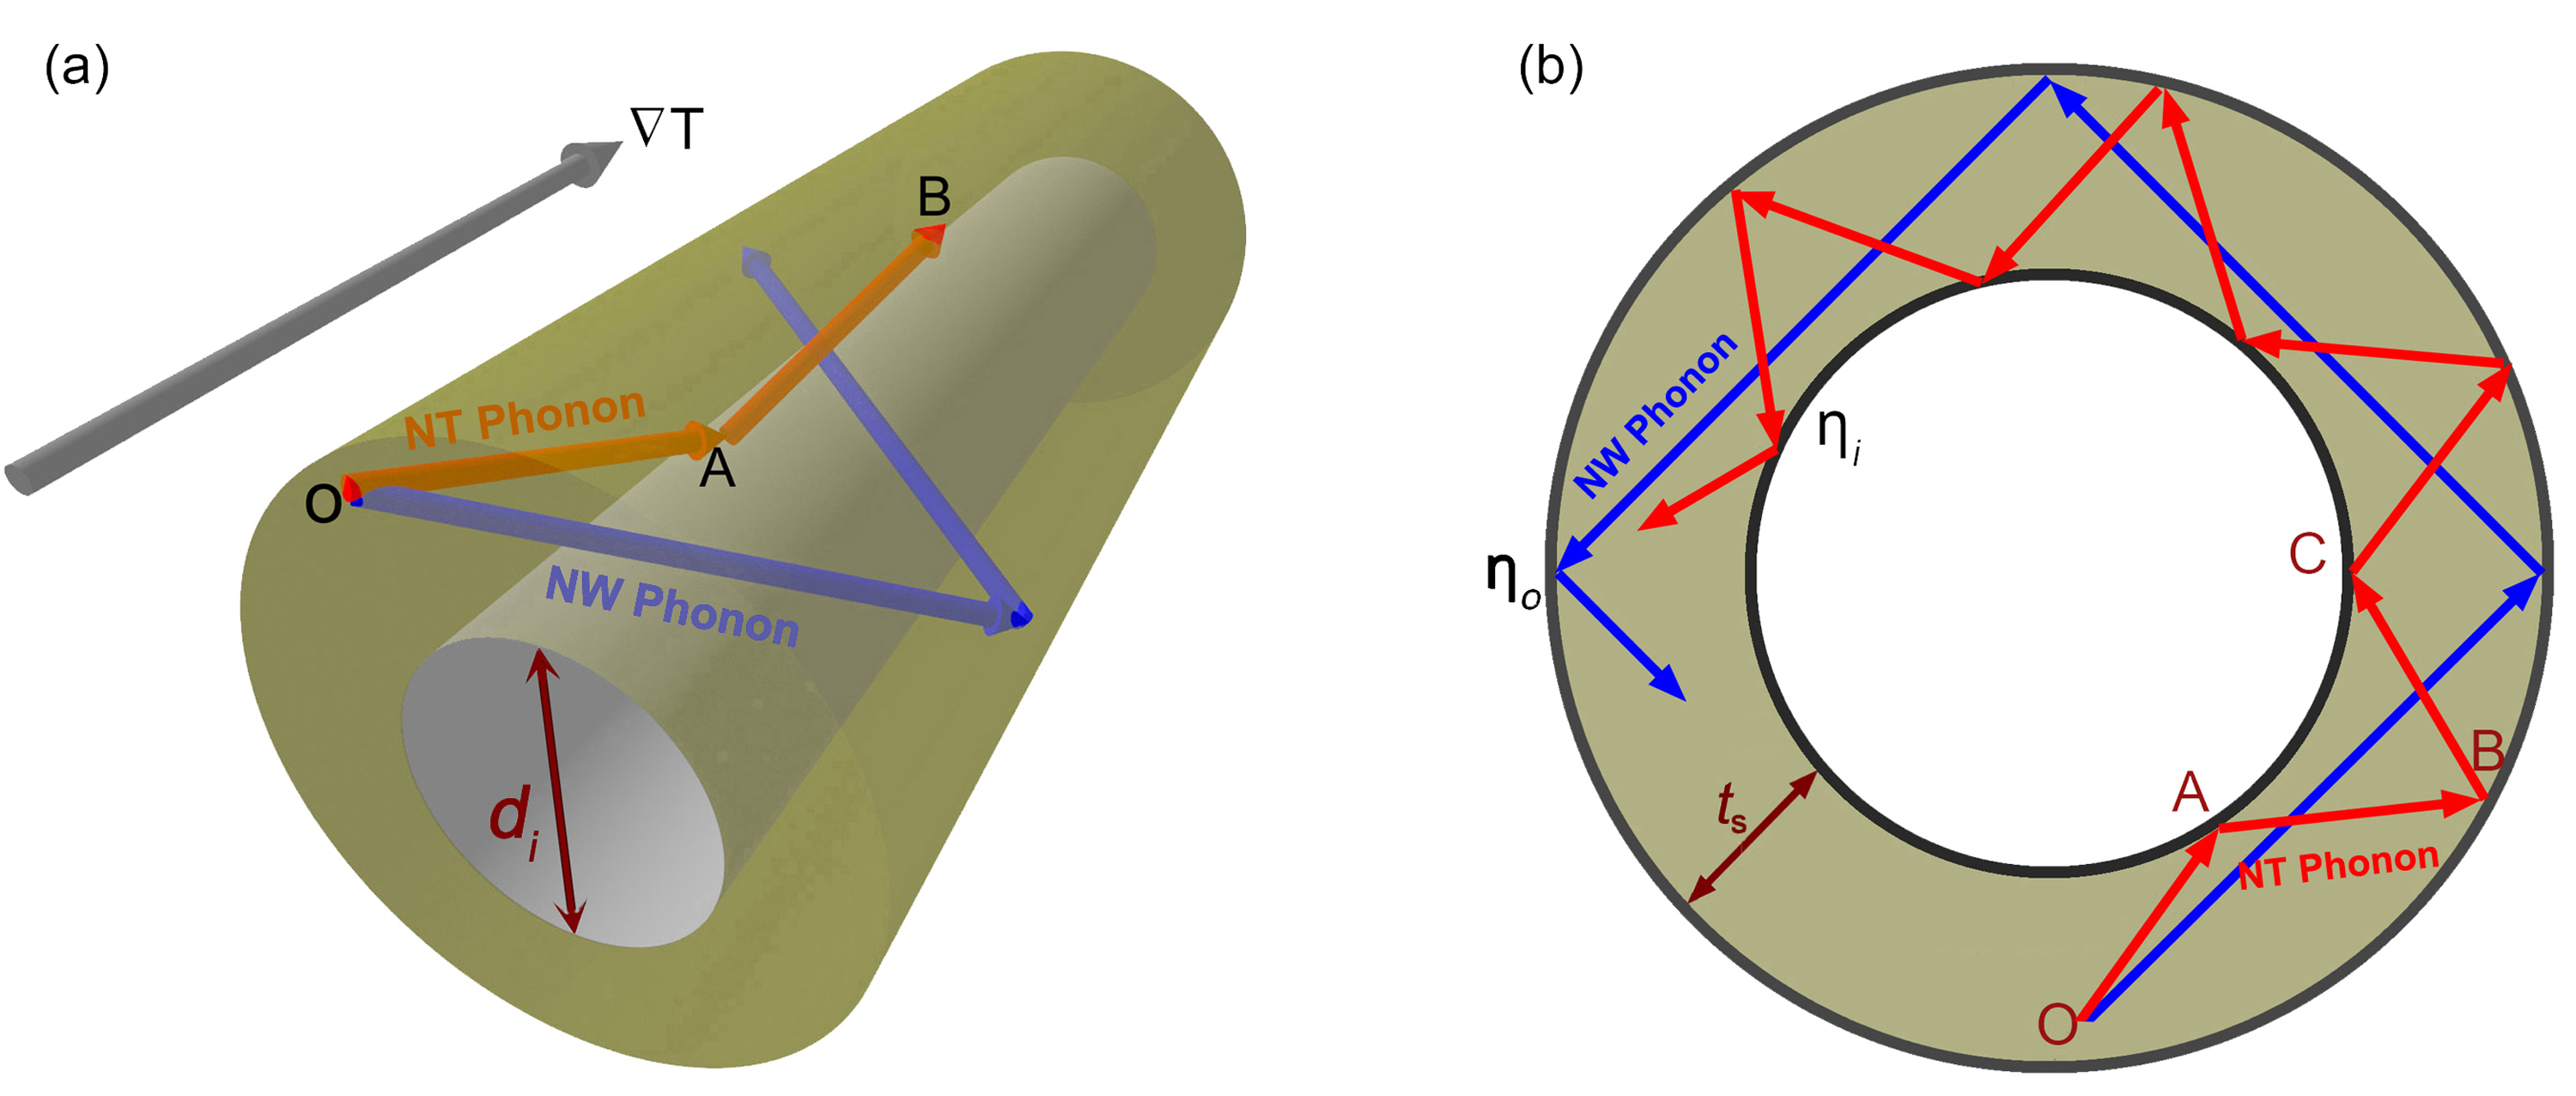
\includegraphics[width=0.95\textwidth]{/ch4/Figure1.jpg}
	\caption{Schematic representations of NT (red) and NW (blue) phonons within a nanotube. (a) NT phonons interact with both inner and outer surfaces while NW phonons interact only with the outer surface. (b) Cross-sectional view of the nanotube with the projections of the phonon trajectories.}
	\label{fig:nt_schematic}
\end{figure}

We show in \Cref{fig:nt_schematic}, a nanotube with inner diameter \gls{di} and outer diameter \gls{do}, creating a silicon shell of thickness \gls{ts}. We note that in a nanotube there are inner and outer surface boundaries which in general can have distinct characteristics from each other. Phonons in nanotubes can be classified on the basis of the presence (or absence) of interaction with the inner boundary based on their angle of propagation and point of origin O within the nanowire. \emph{Phonons that interact with both the inner and outer boundaries are termed as NT phonons and are shown with red arrows, while phonons that propagate unperturbed by the presence of the inner silicon-air interface are termed as NW phonons and shown with blue arrows}. The thermal gradient is applied along the axial direction of the nanotube. \Cref{fig:nt_schematic}(b) is the two-dimensional projection of the phonon transport within a nanotube showing the successive reflections of phonons at the surfaces for both NT and NW phonons. At each of these phonon-surface interactions, part of the thermal energy is specularly reflected while part is lost due to diffusive phonon scattering occurring at the surfaces. We note that our model can selectively incorporate this fundamental difference between the propagation properties of NT and NW phonons in addition to the specific surface scattering properties at the internal and external boundaries. Prediction of thermal transport properties such as thermal conductivity in nanotubes requires analysis of both NT and NW phonon contributions to thermal energy transport. The thermal transport properties of NT phonons are captured via a novel formalism accounting for the reduction in their mean-free-paths upon interaction with the inner and outer boundaries each with its individual specularity \gls{p}$_{in}$ and \gls{p}$_{out}$, respectively. Note that this model of NT phonons is directly derived from the method for asymmetric thin-films shown in \Cref{sec:ch3-method}. At every phonon-outer boundary scattering, $1 - $\gls{p}$_{out}$ proportion of phonons are scattered diffusively, while $1 - $\gls{p}$_{in}$ are diffusively scattered at the inner boundary. For NT phonons with initial propagation direction towards the outer nanotube boundary, the reduced phonon mean-free-paths are calculated as follows,

%Equations here


%\begin{equation}
\begin{align}\label{eq:nt_mode}
\ell_{\vec{k},r,\theta,\textrm{surface-properties}}^{\textrm{NT-mode}} =
&\overbrace{ \int_{0}^{\Lambda}{\frac{r}{\ell_{\vec{k}}^{\textrm{bulk}}}e^{-\frac{r}{\ell_{\vec{k}}^{\textrm{bulk}}}}\,dr} +(1-p_{\textrm{out}})\int_{\Lambda}^{\infty} {\frac{\Lambda}{\ell_{\vec{k}}^{\textrm{bulk}}}e^{-\frac{r}{\ell_{\vec{k}}^{\textrm{bulk}}}}\,dr} }^\text{1st Scattering Event}  \nonumber \\
+&\overbrace{p_{\textrm{out}} \int_{\Lambda}^{\Lambda+\Lambda^{*}}{\frac{r}{\ell_{\vec{k}}^{\textrm{bulk}}}e^{-\frac{r}{\ell_{\vec{k}}^{\textrm{bulk}}}}\,dr} +p_{\textrm{out}}(1-p_{\textrm{in}})\int_{\Lambda+\Lambda^{*}}^{\infty} {\frac{\Lambda+\Lambda^{*}}{\ell_{\vec{k}}^{\textrm{bulk}}}e^{-\frac{r}{\ell_{\vec{k}}^{\textrm{bulk}}}}\,dr} }^\text{2nd Scattering Event}\nonumber \\
+&\overbrace{p_{\textrm{out}}p_{\textrm{in}} \int_{\Lambda+\Lambda^{*}}^{\Lambda+2\Lambda^{*}}{\frac{r}{\ell_{\vec{k}}^{\textrm{bulk}}}e^{-\frac{r}{\ell_{\vec{k}}^{\textrm{bulk}}}}\,dr} +p_{\textrm{out}}p_{\textrm{in}}(1-p_{\textrm{out}})\int_{\Lambda+2\Lambda^{*}}^{\infty} {\frac{\Lambda+2\Lambda^{*}}{\ell_{\vec{k}}^{\textrm{bulk}}}e^{-\frac{r}{\ell_{\vec{k}}^{\textrm{bulk}}}}\,dr} }^\text{3rd Scattering Event}\nonumber \\
+&{\dots}
\end{align}
%\end{equation} 
%!!!!!!!!!!!

where the specularities $p_{in}$ and $p_{out}$ of inner and outer nanotube surfaces depend on \gls{k}, \gls{r}, \gls{eta}, and \gls{cl} i.e. phonon wave number and angle of propagation \gls{theta}, spatial position along the propagation direction, surface roughness and correlation length, respectively. The symbols $\Lambda = OA$, $\Lambda^{*} = AB (=BC)$ correspond to the distances depicted in \Cref{fig:nt_schematic}(b). The reduced mean-free-paths for phonons with their initial propagation direction towards the inner surface can be analogously evaluated by exchanging $p_{in}$ and $p_{out}$ in \Cref{eq:nt_mode}. Note that the sum over infinitely large number of scattering events determines the reduced mean-free-path of the NT phonons. In contrast to NT phonons, the thermal transport properties of NW phonons, as their name suggests, are similar to those in nanowires (see \Cref{chap:predictive}) since in this case the phonons are unperturbed by the presence of the inner boundary of the nanotube [blue modes in \Cref{fig:nt_schematic}(b)]. For NW phonons, a simpler expression for the reduced mean-free-paths can be obtained similar to \Cref{eq:ch2-mfp_reduced}.

The interaction of phonons with the nanostructure boundaries is the key factor that allows for a control over thermal transport properties at the nanoscale and their modification from bulk values. The influence of boundaries on thermal transport becomes stronger with reducing dimensions and the corresponding increase in surface-to-volume ratio. Thus, it is imperative to consider rigorous descriptions of phonon-boundary scattering to accurately predict thermal phonon transport. To describe the phonon-boundary interaction in the nanotube, we use the Beckmann-Kirchhoff surface scattering model and surface shadowing approach (detailed in \Cref{sec:BK}) to determine the surface specularity \gls{p}, which is the proportion of phonons that are specularly reflected upon interacting with a boundary (the proportion $1-p$ is diffusely scattered).

\section{Results and Discussion}
\subsection{Role of Shell Thickness}
A key indicator of phonon transport in nanostructures is the surface-to-volume ratio, and for nanotubes it is inversely proportional to the shell thickness \gls{ts}. Thus, we start our analysis by quantifying the impact of shell thickness on thermal conductivity \gls{K} by considering a pure Si nanotube and two silicon-germanium alloy nanotubes -- \sige{0.90}{0.10}, \sige{0.95}{0.05}, all with fixed outer diameter \gls{do} of 100 nm [\Cref{fig:nt_fig2}]. The outer diameter selection is similar to previously experimentally grown crystalline nanotubes \cite{RN436}. We fix the correlation length \gls{cl} to be ten times the roughness \gls{eta} for simplicity in analysis \cite{ownNW}.  We also consider bulk dispersion relations apply, as the coherent effects and quantum confinement are expected to be small at the temperature and structural conditions (thickness and roughness scales) considered in this study \cite{RN240,RN447}. Additionally, for the scattering from small proportion of Ge atoms in a Si host, we use effective medium approach based on Rayleigh scattering of phonons from a virtual crystal of Si and alloyed Ge. This approach has been shown to accurately provide the bulk SiGe thermal conductivity dependence on alloying with Ge \cite{RN132,RN289}. 

% Fig2
\begin{figure}[hbt]
	\centering 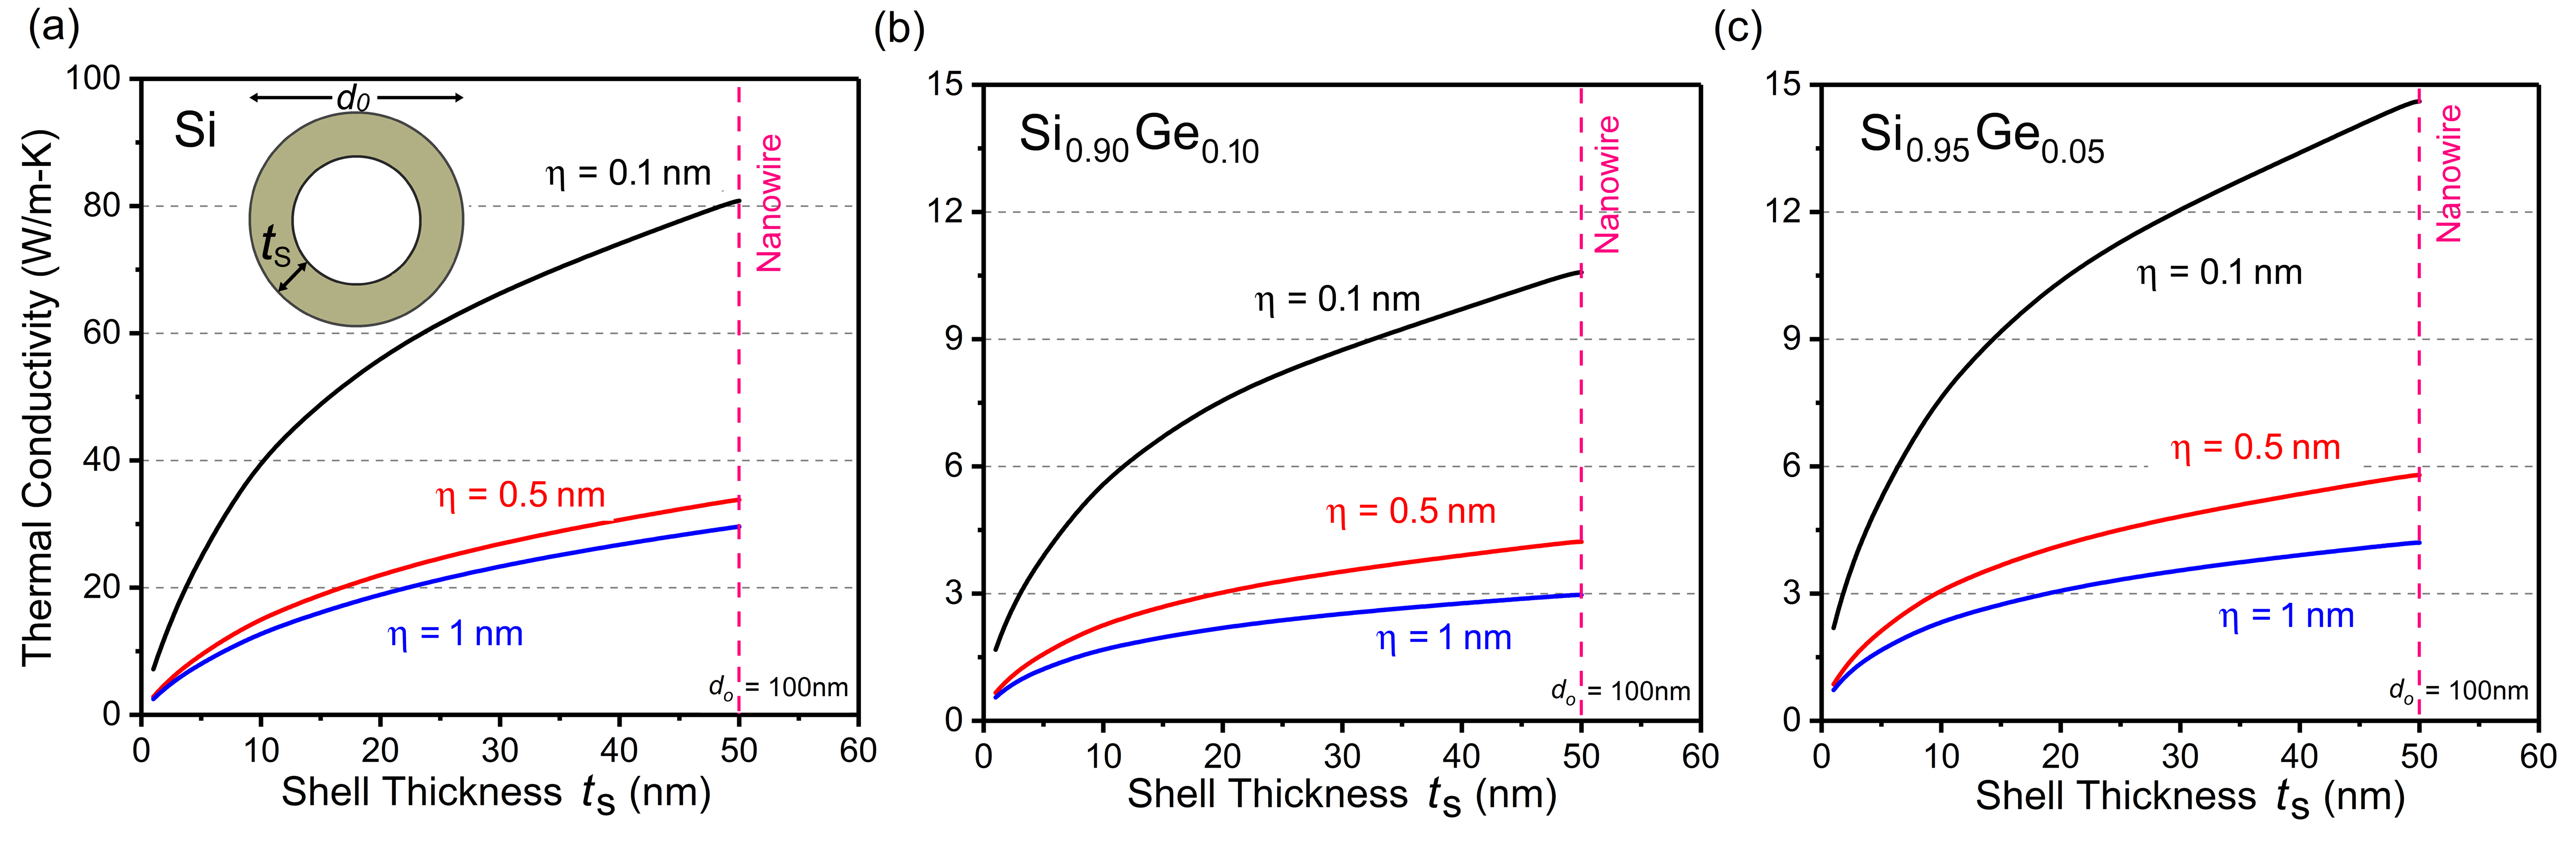
\includegraphics[width=\textwidth]{/ch4/Figure2.jpg}
	\caption{Thermal conductivity of nanotubes at room temperature as a function of shell thickness \gls{ts} for (a) crystalline silicon, (b) silicon nanotubes with 10\% alloyed germanium, and (c) silicon nanotubes with 5\% alloyed germanium. The outer diameter \gls{do} is 100 nm and the inner and outer boundaries are assumed to have identical surface properties \gls{eta}.}
	\label{fig:nt_fig2}
\end{figure}

We show in \Cref{fig:nt_fig2} how for all the cases increasing surface roughness reduces the thermal conductivity of the nanotube due to more diffusive scattering of phonons at boundaries. Additionally, we show that the reduction in nanotube shell thickness leads to a decreasing thermal conductivity owing to the increased surface-to-volume ratio. Note that, in contrast to nanowires, nanotubes provide an avenue to access lower thermal conductivity regimes even with large experimentally realizable outer diameters, making them a promising candidate for low thermal conductivity applications.


\subsection{Predictions of Thermal Spectra}

\begin{figure}[b!]
	\centering 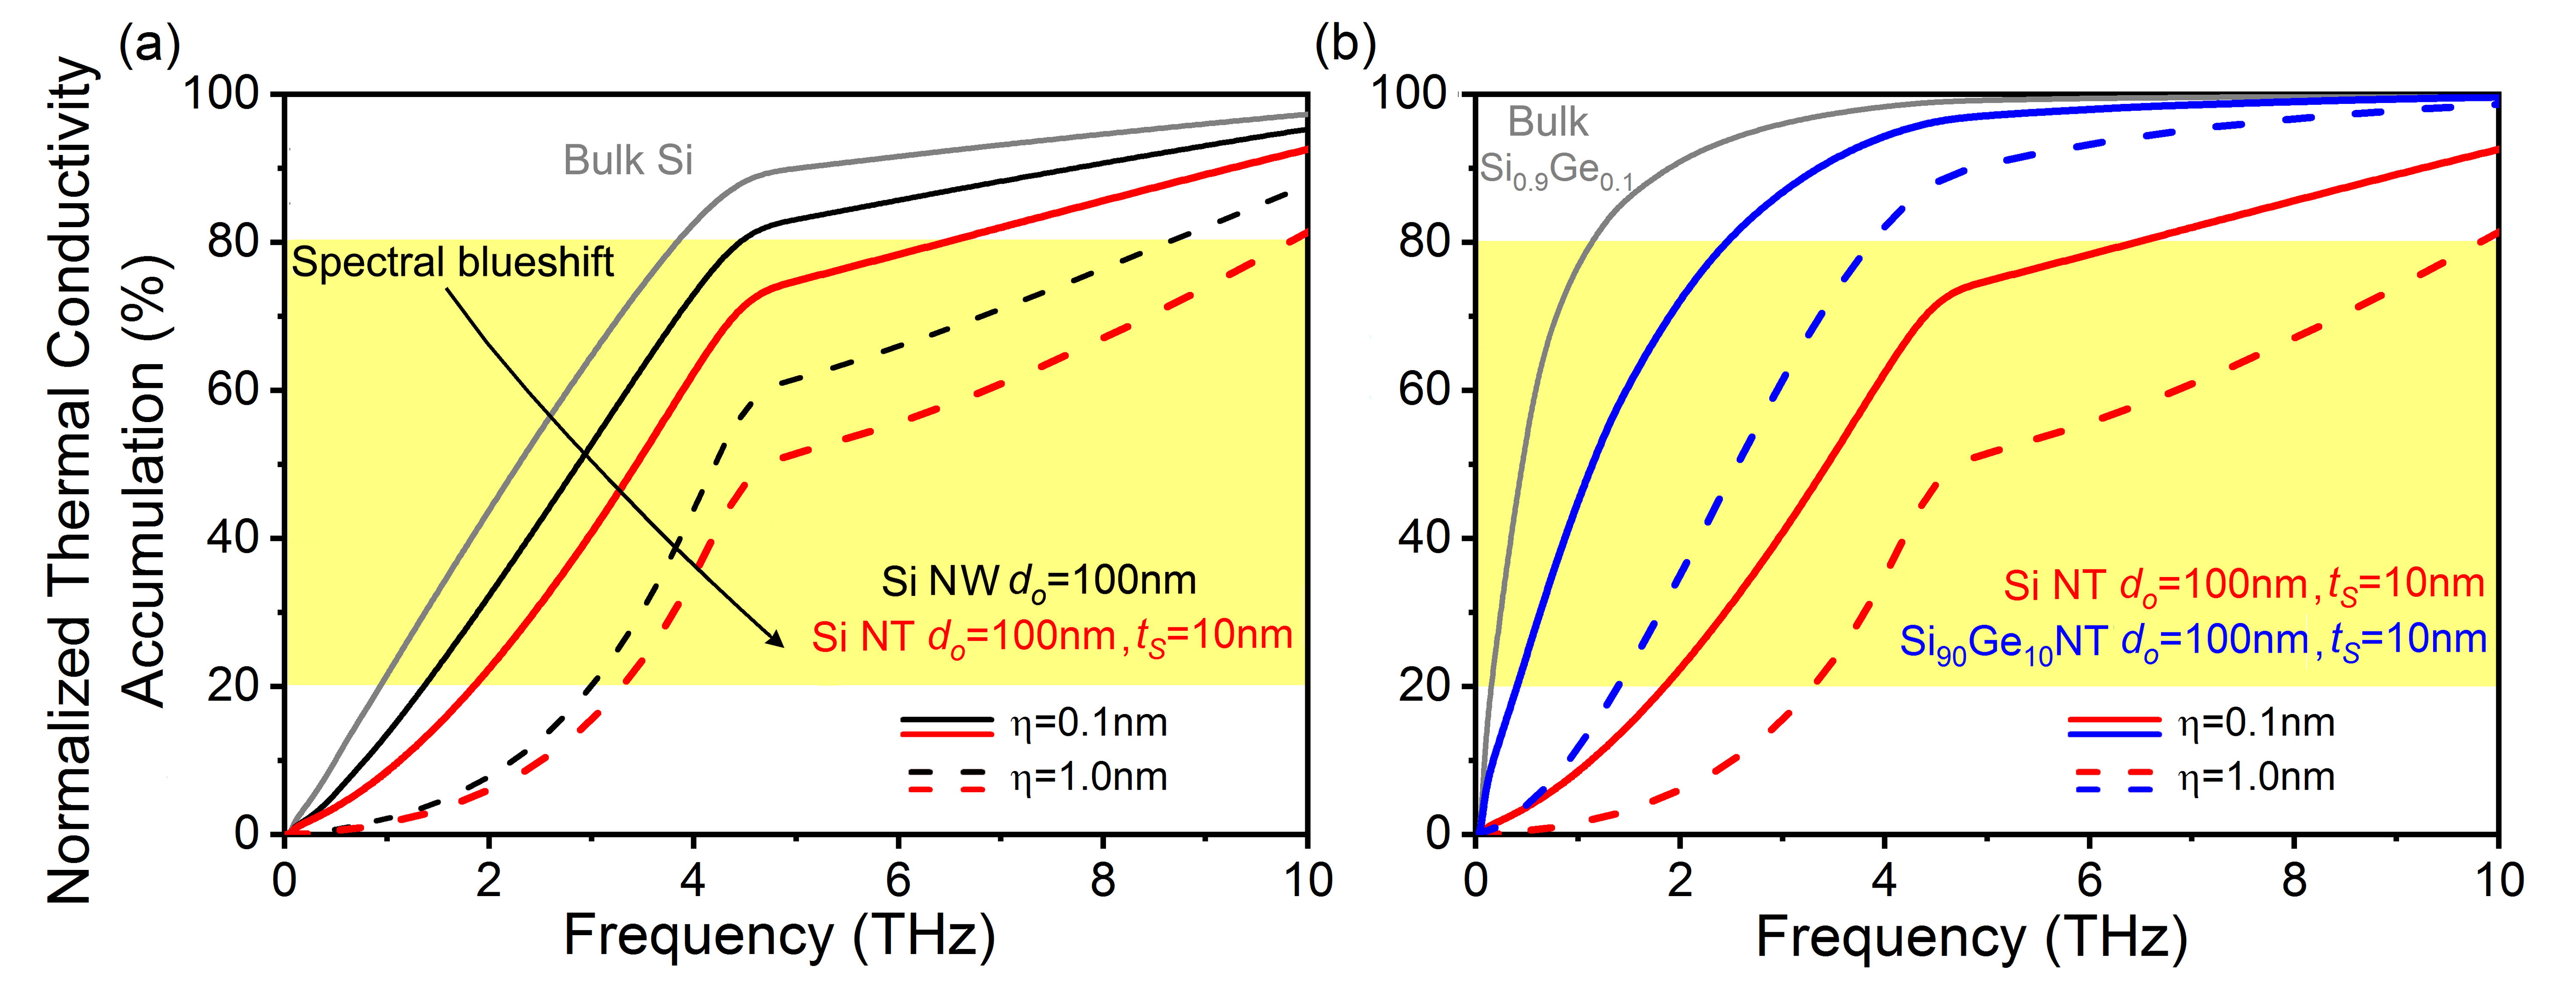
\includegraphics[width=\textwidth]{/ch4/Figure3.jpg}
	\caption{Frequency heat-spectra (or normalized thermal conductivity accumulation functions) for (a) bulk Si (gray line), 100 nm diameter Si nanowires (black), and Si nanotubes of outer diameter 100 nm and shell thickness 10 nm (red) at room temperature. The effect of alloying is shown in (b) where the spectra for bulk \sige{0.90}{0.10} is shown in gray and for an alloyed nanotube in blue. Si nanotubes are shown for reference in red as in (a). The solid and dotted lines represent surface roughnesses of \gls{eta} = 0.1 and \gls{eta} = 1.0 nm.}
	\label{fig:nt_fig3}
\end{figure}

\begin{figure}[b!]
	\centering 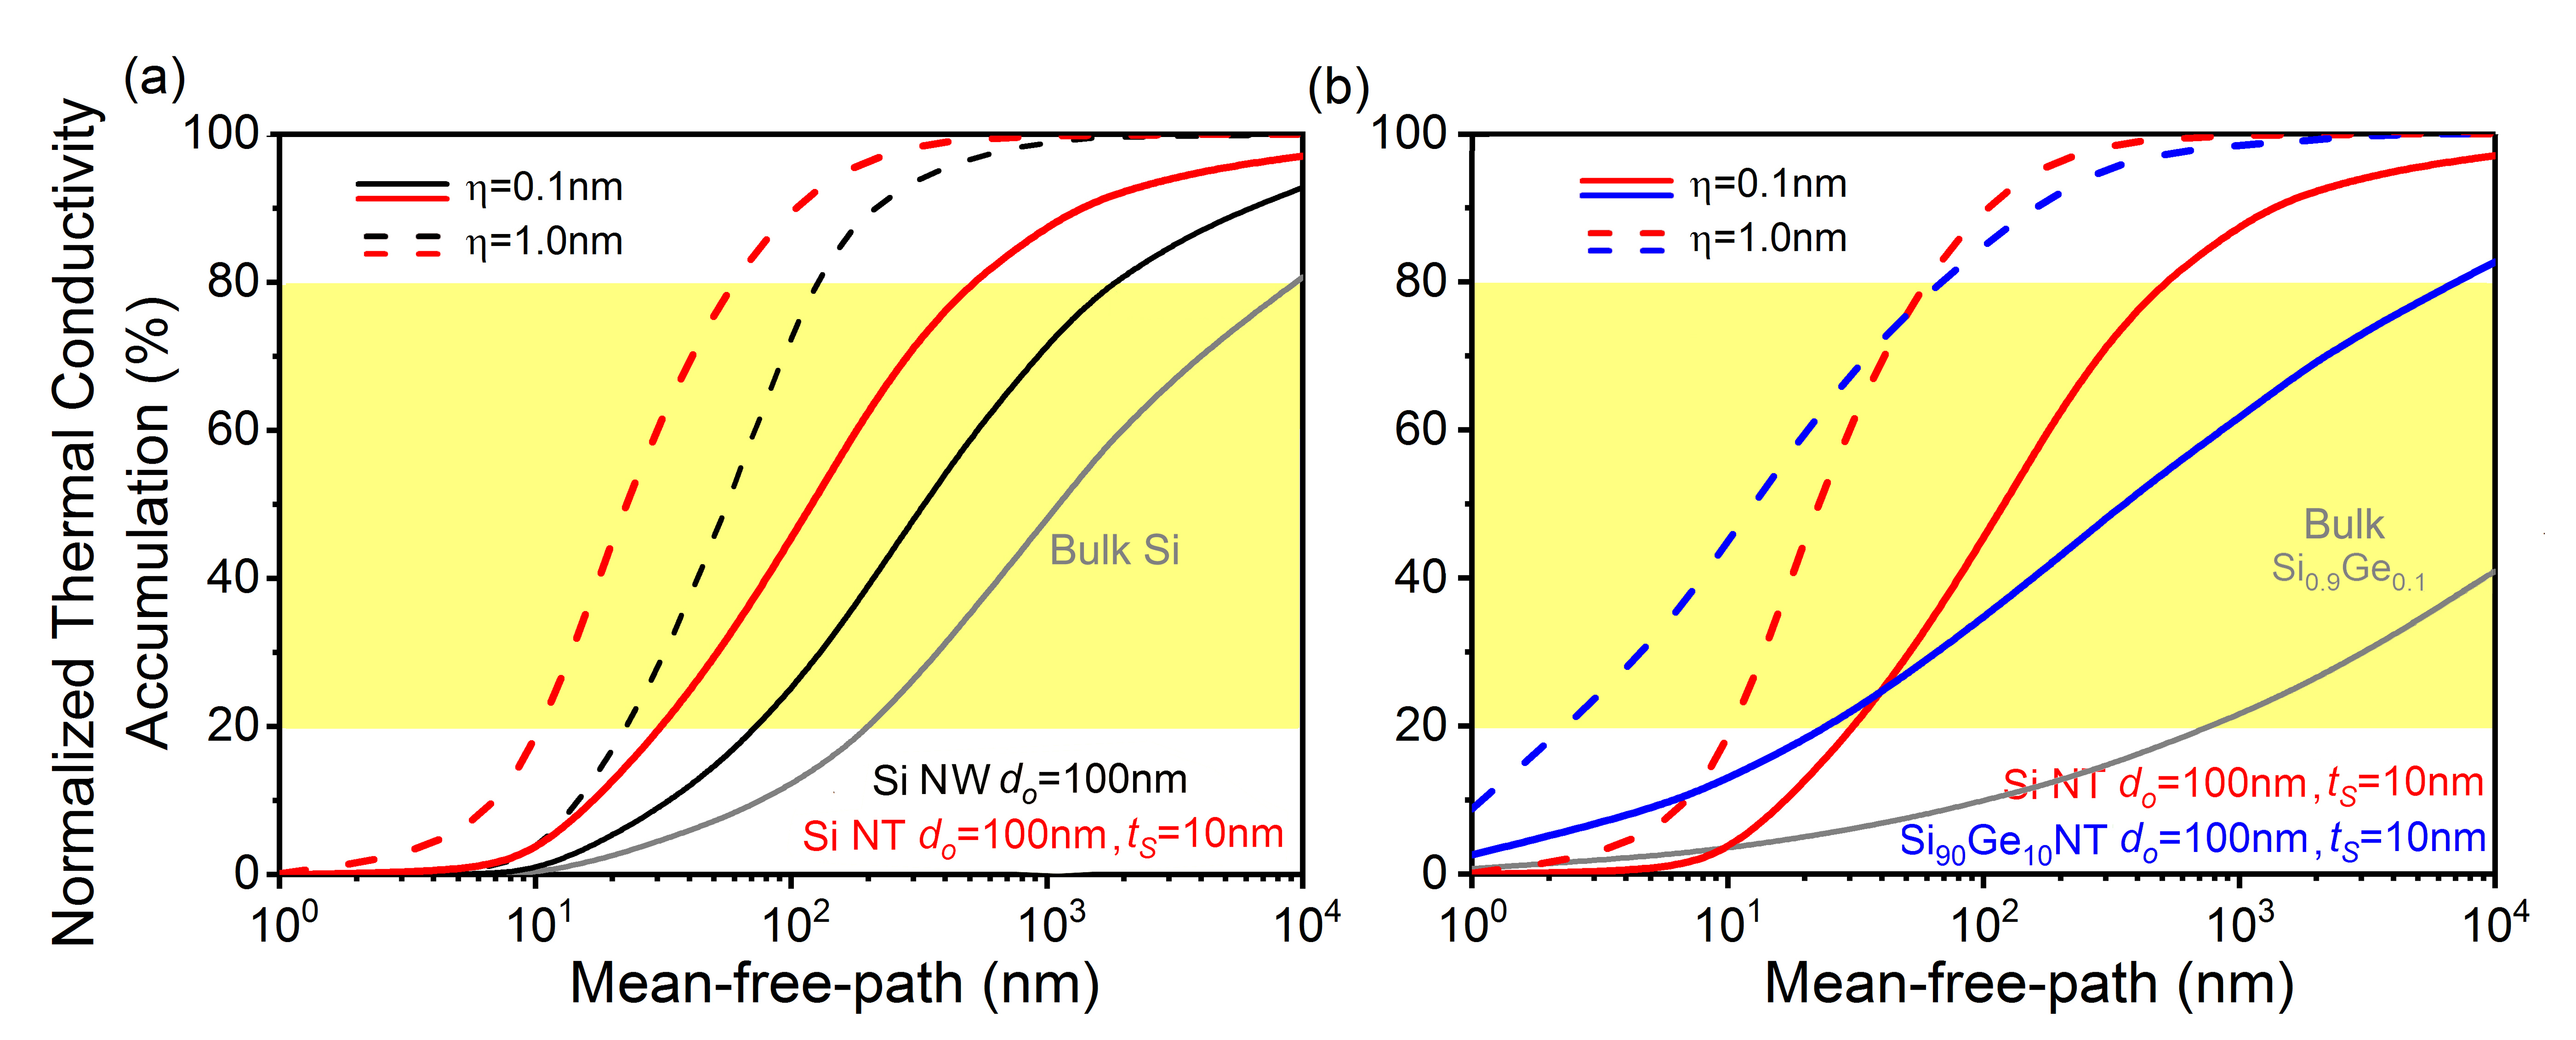
\includegraphics[width=\textwidth]{/ch4/Figure4.jpg}
	\caption{Mean-free-path heat spectra for (a) Si nanotubes (red) and nanowires (black) and (b) Si (red) and \sige{0.90}{0.10} nanotubes (blue) at \gls{T} = 300 K. Solid and dotted lines represent surface roughnesses of \gls{eta} = 0.1 nm and \gls{eta} = 1.0 nm, respectively. Bulk heat spectra are shown in gray.}
	\label{fig:nt_fig4}
\end{figure}

To elucidate the thermal transport mechanisms in nanotubes and understand the effects of impurity atoms in host lattice and surfaces, we next predict and analyze the frequency and mean-free-path thermal conductivity accumulation functions for several different structural and physical nanotube conditions. These heat spectra are the foundational basis for designing thermal materials for targeted applications (see \Cref{sec:pred_thermalspectra}). Starting with bulk Si, our calculations show that at room temperature, the addition of alloy atoms impacts the amount of heat carried by high frequency phonons strongly, moving the middle 60\% of heat spectra from the range 1–4 THz [\Cref{fig:nt_fig3}(a), solid gray line] to low frequency phonons with frequencies $<$ 1 THz [\Cref{fig:nt_fig3}(b), solid gray line]. That is, there is \emph{red shift} in the phonon frequency spectrum. The mean-free-path spectra for bulk Si [\Cref{fig:nt_fig4}] shows a corresponding shift towards larger mean free paths when Ge alloy atoms are present. We note that with Ge alloying, phonons with smaller mean-free-paths (also, higher frequencies) 	are scattered efficiently due to Rayleigh scattering by impurities (i.e. $\tau\!\sim\!\omega^{4}$), causing the proportion of heat transported by large mean-free-path phonons to increase. For example, we find that for alloyed nanotubes with smooth surfaces, 20\% of heat is carried by phonons of mean-free-paths larger than 10 $\mu$m in agreement with results from nanowires (see \Cref{chap:predictive}). In addition to alloying, surface scattering provides an extra degree to further tailor the frequency and mean-free-path heat spectra. For example, a Si nanowire of outer diameter \gls{do} = 100 nm and roughness \gls{eta} = 0.1 nm [\Cref{fig:nt_fig3}(a), solid black line] has its heat spectra blue-shifted to high frequencies with respect to bulk silicon [\Cref{fig:nt_fig3}(a), solid gray line]. The corresponding mean-free-path spectra moves towards smaller mean-free-paths. This blue-shift in heat spectra arises due to the presence of phonon-boundary scattering, which primarily reduces the mean-free-path of low-frequency phonons since high-frequency phonons have short mean-free-path phonons and are not able to interact with the boundaries. Importantly, nanotubes allow leveraging the phonon-boundary scattering mechanisms to strongly manipulate the heat spectra. For instance, a Si nanotube of the same outer diameter \gls{do} of 100 nm and roughness 0.1 nm on inner and outer boundaries and with a shell thickness \gls{ts} = 10 nm [\Cref{fig:nt_fig3}(a) and \Cref{fig:nt_fig4}(a), solid red line] shows a stronger blue shift to higher frequencies and shorter mean-free-paths than a nanowire of the same outer diameter. Furthermore, the effect of increasing roughness tends to blue shift the spectra to high frequencies as evidenced by the spectra of a nanotube with 1 nm roughness on both inner and outer boundaries \Cref{fig:nt_fig3}(a) and \Cref{fig:nt_fig4}(a), dashed red line]. Small surface roughness is therefore more appropriate from a thermal wave-effect perspective, as lower frequencies and larger mean-free-paths are better suited for coherent phonon manipulation in nanostructured materials. Note that SiGe alloy nanotubes can help to reduce the thermal phonon frequencies with respect to Si nanotubes [\Cref{fig:nt_fig3}(b), blue vs red lines], while preserving a long range of mean-free-paths [\Cref{fig:nt_fig4}(b), blue lines]. For instance, in Si NT with surface roughness \gls{eta} = 1 nm, the middle 60\% of heat is carried by phonons of $\sim$ 3–10 THz frequency range and 10–60 nm mean-free-path range. With alloying, the frequency range red-shifts to 1.5–4 THz, while mean-free-paths shift to 3–70 nm.


\subsection{Role of Different Inner and Outer Surface Conditions}

\begin{figure}[t!]
	\centering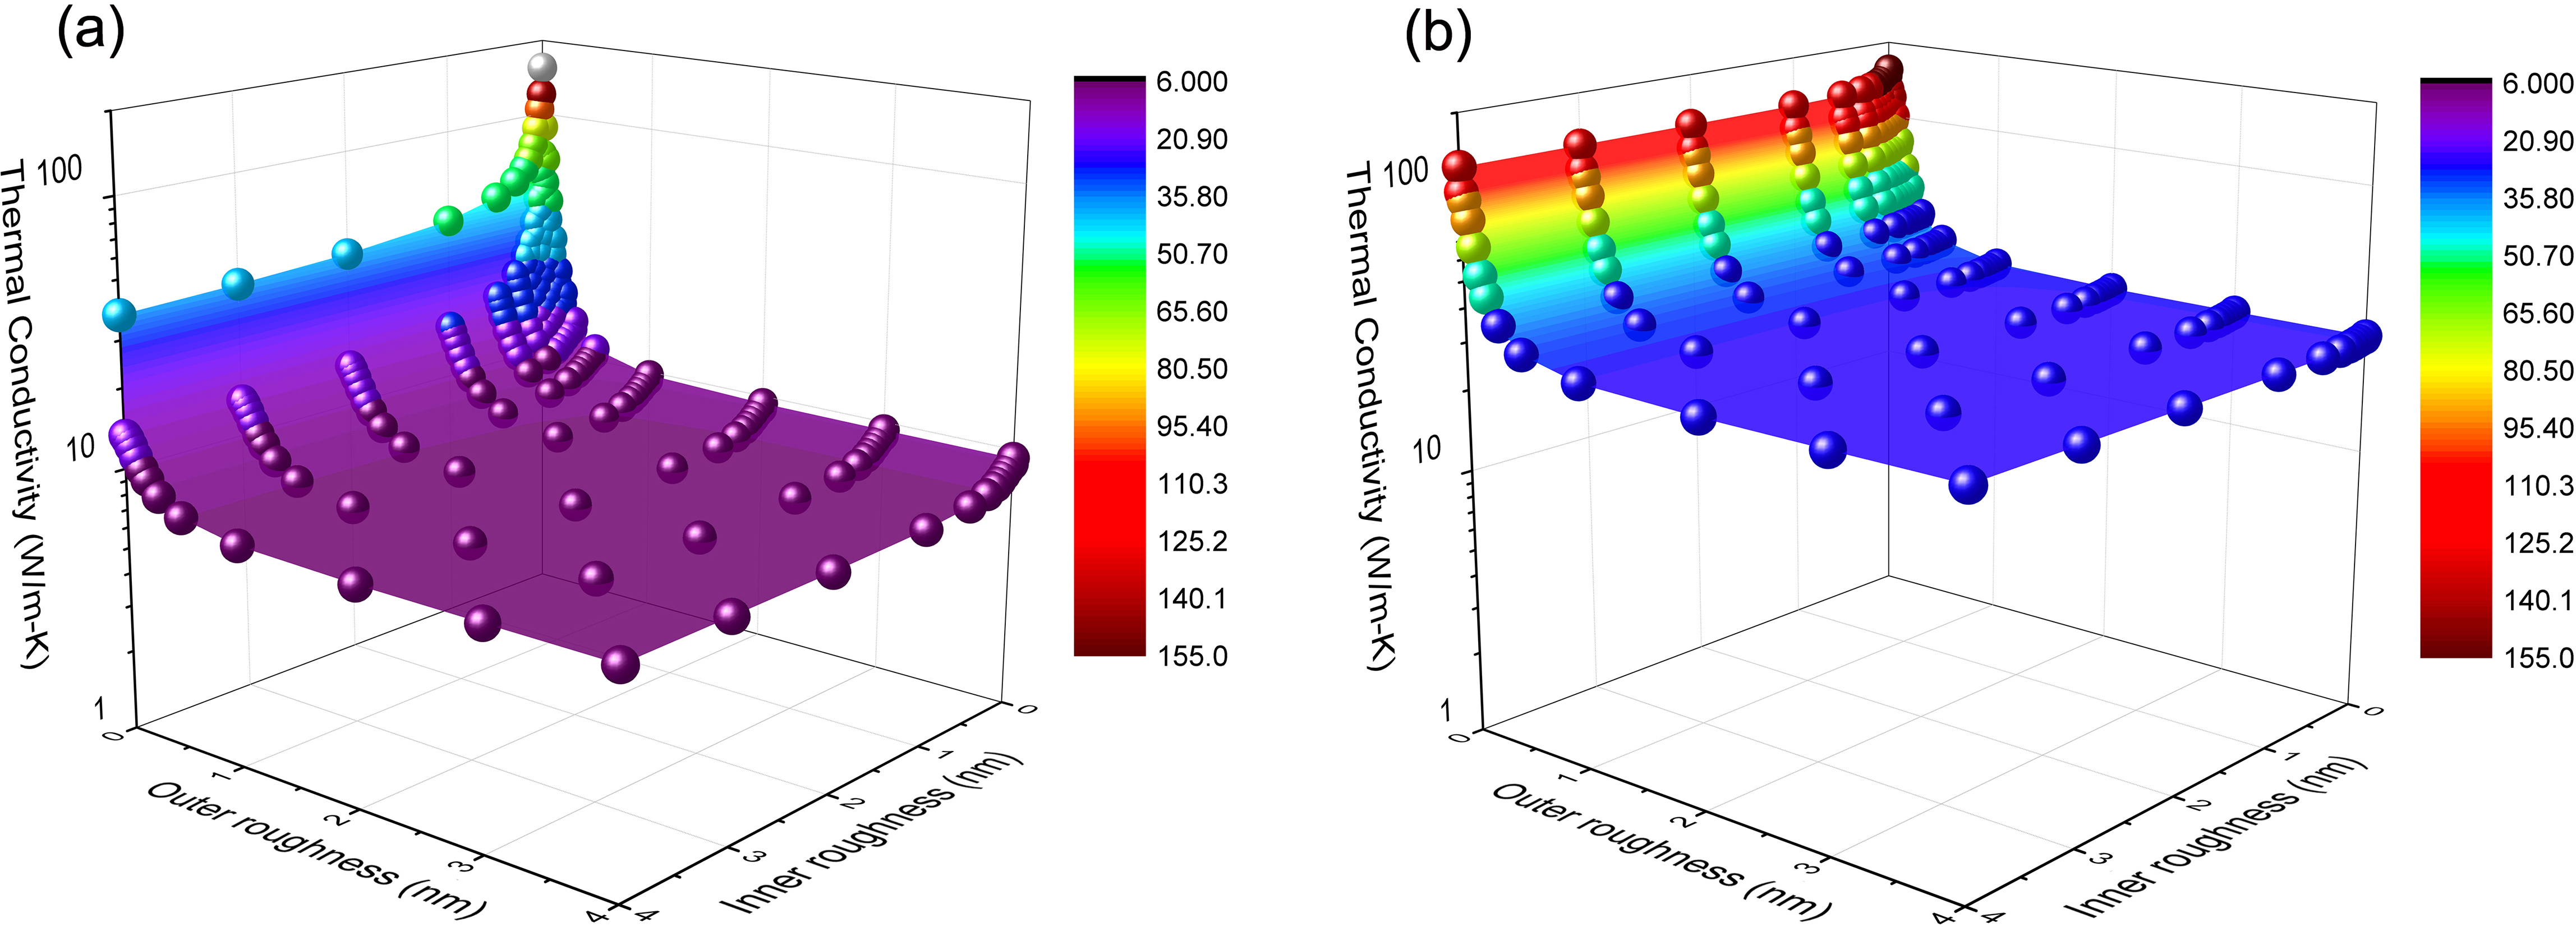
\includegraphics[width=\textwidth]{/ch4/Figure6.jpg}
	\caption{Thermal conductivity of Si nanotubes as a function of both inner and outer surface roughness \gls{eta}$_{in}$ and \gls{eta}$_{out}$ with (a) shell thickness \gls{ts} = 4 nm and (b) shell thickness \gls{ts} = 40 nm. Both nanotubes have outer diameter \gls{do} = 100 nm.}
	\label{fig:nt_fig6}
\end{figure}

Since in general the inner and outer surface nanotube surfaces could be exposed to different processing conditions, we next study phonon thermal transport in nanotubes where the inner and outer surfaces have different roughnesses. We consider two nanotubes: a thin shell nanotube with \gls{ts} = 4 nm and a thicker nanotube with \gls{ts} = 40 nm. The outer diameter for the thin shell nanotube is \gls{do} = 100 nm, similar to experimental grown nanotubes \cite{RN436}. The choice of these nanotubes allows for an analysis over a wide spectrum of structural dimensions. For a thin-shell nanotube (i.e. \gls{ts} = 4 nm) [\Cref{fig:nt_fig6}(a)] the thermal conductivity is more affected by the inner roughness in contrast to a nanotube with thicker outer shell (i.e., \gls{ts} = 40 nm) [\Cref{fig:nt_fig6}(b)]. The differential influence of inner boundary properties on thermal conductivity arises due to higher number of NT phonons in a thinner shell nanotube than a thicker nanotube. In a thicker shell nanotube, NW phonons, which remain unperturbed by the presence of inner surface conditions, are in higher proportions. It can also be observed that the thermal conductivity of Si nanotubes reduces with increasing roughness of surfaces, approaching a saturation roughness (or asymptotic behavior) indicative of the onset of nearly fully diffusive surface ($p_{in}\sim p_{out}\sim 0$). The saturation roughness is expected to be a function of the temperature following the mean-free-path heat spectra described previously. At room temperature this saturation roughness value is found to be in the order of \gls{eta} $\sim$ 2 nm. 

\begin{figure}[hbt]
	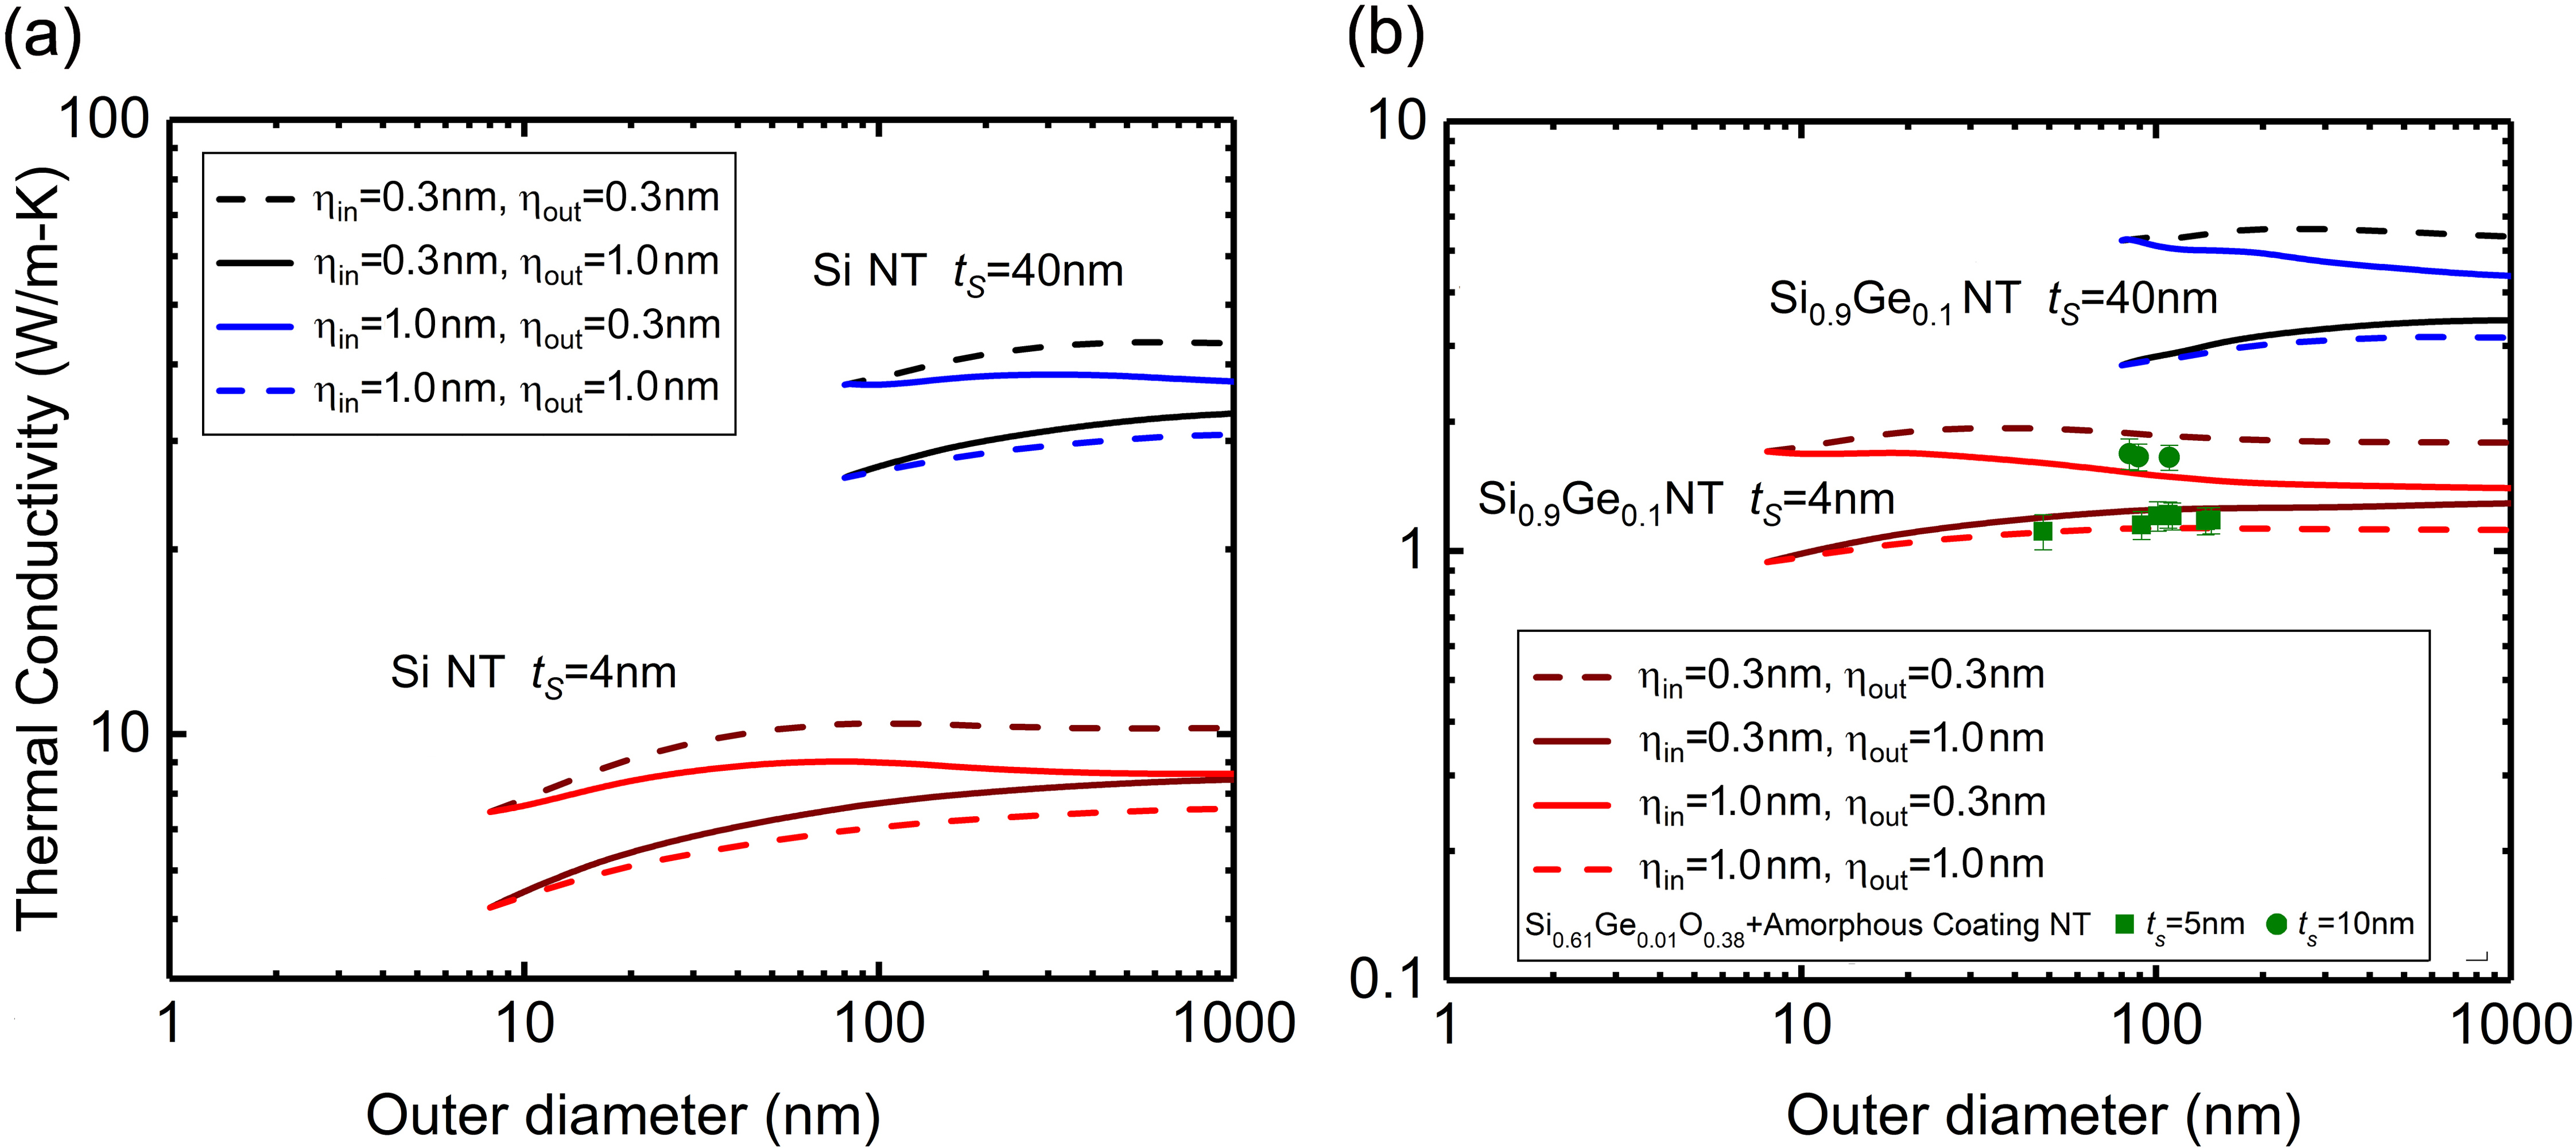
\includegraphics[width=\textwidth]{/ch4/Figure7.jpg}
	\caption{The thermal conductivity for (a) Si nanotubes and (b) \sige{0.90}{0.10} nanotubes as a function of outer diameter with varying surface roughnesses. Black and blue lines correspond to thicker shell (\gls{ts} = 40 nm) nanotube while wine and red lines correspond to thinner shell nanotube (\gls{ts} = 4 nm).}
	\label{fig:nt_fig7}
\end{figure}

To understand the correlation between the outer diameter, surface properties, and thermal conductivity, we next fix the shell thickness \gls{ts} as 4 nm and 40 nm while varying the outer diameter for Si [\Cref{fig:nt_fig7}(a)] and \sige{0.90}{0.10} [\Cref{fig:nt_fig7}(b)] nanotubes. The starting point of every curve at small outer diameters corresponds to the thermal conductivity when the inner diameter approaches zero (i.e. when the nanotube approaches a nanowire). In both Si and \sige{0.90}{0.10} nanotubes, the effect of a higher surface roughness leading to a lower thermal conductivity than smoother surface nanotube is observed. The thermal conductivity for the cases with two surfaces having distinct roughnesses (solid lines) are different from one another and show differential sensitivity to changing outer diameter highlighting the role of individual properties. The conductivity behavior with diameter in both these cases is a consequence of changing proportion of NT and NW modes in these structures, since for a fixed shell thickness, a larger outer diameter causes more phonons to interact with the inner surface transforming more NW phonons to NT phonons. We note that the sensitivity of thermal conductivity to increasing outer diameter for thin nanotubes is diminished as they begin to approach a ‘thin-film’ like structure \cite{RN431}.

\section{Summary}
We analyzed the behavior of thermal energy transport in an emerging class of one-dimensional nanomaterials viz. semiconductor nanotubes. Using frequency-dependent phonon properties and quantifiable surface properties, we presented a rigorous physical description of heat conduction that captures the underlying phonon dynamics in these novel nanostructures. Our model allowed us to evaluate nanotube thermal conductivities for a wide range of material and structural properties including alloying, outer diameters, shell thicknesses and temperatures; \emph{while preserving the ability to treat the two surfaces independently with their distinct roughnesses}. The independent treatment of the two surfaces was used to explain their differential role in thermal transport in these nanostructures. We concluded that in general, the thermal conductivity of the nanotube depends on the outer diameter even for the same shell thickness. We showed that the experimentally observed independence between these quantities could be explained by a combination of addition of impurity atoms to the Silicon lattice and surface roughness. The frequency and mean-free-path heat spectra showed in this thesis are a critical step towards fully discerning thermal conduction in these nanostructures and moving towards a guided material design. The methodology and the results of this chapter provide a fundamental understanding into thermal transport phenomenon in low-dimensional nanotube structures.





